\subsection{Recap: Size of Configuration Spaces}
\subsection{Costs of Variability}
\subsection{Common Interaction Patterns}
% here or together with Variability Bug Database?
\subsection{Interactions on Data and Control Flow}
% MWK+:ASE16
\subsection{Interactions in Automotive Product Lines}
\subsection{Reduction of Variants as Solution}
\begin{frame}{\myframetitle}
	\leftorright{
		\pic[width=\linewidth]{ford-t-1910}
	}{
		\mynote{Henry Ford, 1909}{\mycite{Any customer can have a car painted any color that he wants so long as it is black.}}
		\myexample{Why only black?\mysource{\fospl}}{
			\begin{itemize}
				\item black color dried faster
				\item faster production
				\item more products and cheaper production
			\end{itemize}
		}
	}
\end{frame}

\subsection{In Practice: Increase of Features and Variants}
% features: Linux
% variants: Automotive02-05, KfW?
\subsection{The Choice of Features}
\subsection{Choose Features Wisely}
\begin{frame}{\myframetitle}
	\leftorright{
		\myexampletight{John Ferguson Smart (2017)}{\pic[width=.98\linewidth,angle=2,trim=0 0 5 0,clip]{unnecessary-features}}
		% 
	}{
		\centering\href{https://commons.wikimedia.org/wiki/File:John_Carmack_at_GDCA_2017_--_1_March_2017_(cropped).jpeg}{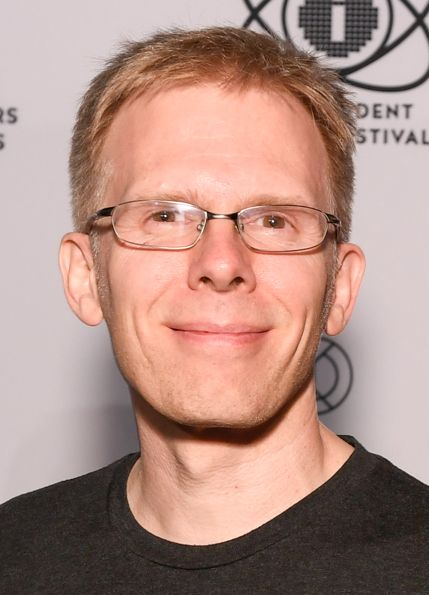
\includegraphics[width=.47\linewidth,trim=0 0 0 0,clip]{john-carmack}}
		\vspace{-7mm}
		
		\mynote{John Carmack (born 1970) \mysource{\href{https://www.ics.uci.edu/~pattis/quotations.html\#C}{uci.edu}}}{\mycite{The important point is that the cost of adding a feature isn't just the time it takes to code it. The cost also includes the addition of an obstacle to future expansion. %Sure, any given feature list can be implemented, given enough coding time. But in addition to coming out late, you will usually wind up with a codebase that is so fragile that new ideas that should be dead-simple wind up taking longer and longer to work into the tangled existing web. 
		[...] The trick is to pick the features that don't fight each other.}}
		% video game developer, co-founder of a video game company
	}
\end{frame}

\subsection{Document Interactions: Incompatibilities of Lenovo Hardware}
\begin{frame}{\myframetitle}
	\begin{mycolumns}[widths={55}]
		\begin{note}{Documentation of Remaining Interactions}
			\begin{itemize}
				\item not all interactions can be prevented/fixed
				\item how to apply strategy S1 (see Part II) if there is no feature model?
				\item what to document?
			\end{itemize}
		\end{note}
		\begin{example}{Lenovo's Option Compatibility Matrices}
			\begin{itemize}
				\item 7 Excel files for current products (+ archive for old products)
				\item Excel file for computers contains 32 tables (series)
				\item table for ThinkPad X has 28 columns (models) and $>500$ rows (accessories)
				\item 14k cells contain $>400$ different footnotes
				\item a footnote explains one incompatibility
			\end{itemize}
		\end{example}
	\mynextcolumn
		\includegraphics[width=\linewidth,page=22,trim=360 20 40 20,clip]{2021/2021-09-08-SPLC-Keynote}
	\end{mycolumns}
\end{frame}
\begin{frame}{\myframetitle}
	\begin{mycolumns}[widths={80},animation=none]
		\includegraphics[width=\linewidth,page=19]{2021/2021-09-08-SPLC-Keynote}
	\mynextcolumn
		\begin{example}{}\setlength\leftmargini{3mm} 
			\begin{itemize}
				\item columns contain notebooks
				\item rows contain acessories
				\item X indicates compatibility
				\item numbers indicate a known incompatibility
			\end{itemize}
		\end{example}
	\end{mycolumns}
\end{frame}
%\begin{frame}{\myframetitle}
%	\centering\includegraphics[height=\textheightwithtitle,page=20]{2021/2021-09-08-SPLC-Keynote}
%\end{frame}
\begin{frame}{\myframetitle}
	\begin{mycolumns}[widths={80},animation=none]
		\includegraphics[width=\linewidth,page=21]{2021/2021-09-08-SPLC-Keynote}
	\mynextcolumn
		\begin{example}{}\setlength\leftmargini{3mm} 
			\begin{itemize}
				\item 314: pen requires touch screen (cf.\ S1)
				\item 315/319/320: extra module needed (cf.\ S6)
				\item 316/317: fixed in newer BIOS versions
				\item 318/321: two modules with a different power supply (cf.\ S3)
			\end{itemize}
		\end{example}
	\end{mycolumns}
\end{frame}

% TODO \subsection{Number of Features in Linux}
%\begin{frame}{\myframetitle\ \mytitlesource{\href{https://www4.cs.fau.de/Ausarbeitung/MA-I4-2015-04-Hengelein.pdf}{Hengelein 2015}}}
%	\partofpage{70}{
%		% TODO \myexampletight{{2005--2015: Number of Features Tripled}}{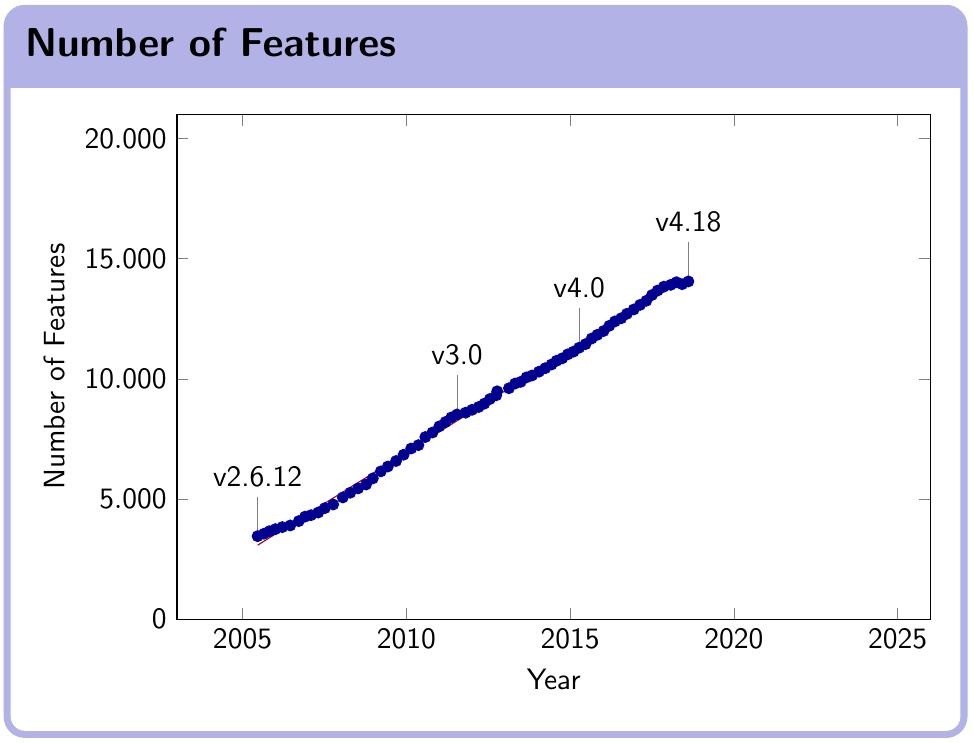
\includegraphics[width=\linewidth]{linux-features}}
%	}
%\end{frame}

% TODO variant reduction, prevent the explosion. marketing wants them all. engineering and quality assurance too expensive.

